\begin{figure}[htp]
  \centering
  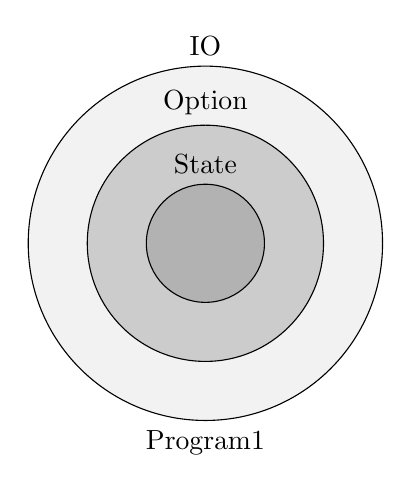
\begin{tikzpicture}
    \node[circle, fill=black!5, draw, minimum size=4.5 cm,label=above:{\lstinline{IO}}, label=below:{\lstinline{Program1}}] {};
    \node[circle, fill=black!20, draw, minimum size=3 cm,label=above:{\lstinline{Option}}] {};
    \node[circle, fill=black!30, draw, minimum size=1.5 cm,label=above:{\lstinline{State}}] {};
  \end{tikzpicture}
  \qquad
  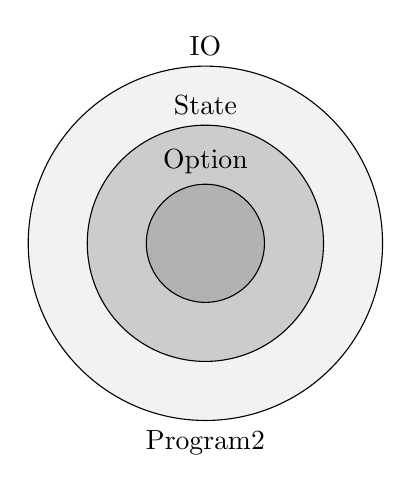
\begin{tikzpicture}
    \node[circle, fill=black!5, draw, minimum size=4.5 cm,label=above:{\lstinline{IO}}, label=below:{\lstinline{Program2}}] {};
    \node[circle, fill=black!20, draw, minimum size=3 cm,label=above:{\lstinline{State}}] {};
    \node[circle, fill=black!30, draw, minimum size=1.5 cm,label=above:{\lstinline{Option}}] {};
  \end{tikzpicture}
  \caption{Rappresentazione grafica degli stack di monadi corrispondenti ai tipi \lstinline{Program1} e \lstinline{Program2}}
  \label{fig:transformers_stacks}
\end{figure}
